\documentclass[10pt]{article}
\usepackage[letterpaper,margin=0.9in]{geometry}
\usepackage{amsmath}
\usepackage[T1]{fontenc}
\usepackage{txfonts}
\usepackage{xcolor,graphicx,booktabs,microtype,enumitem}
\usepackage[font=small,labelfont=bf,margin=0pt]{caption}
\usepackage[colorlinks=true,linkcolor=blue!50!black,urlcolor=blue!50!black]{hyperref}
\setlist{itemsep=2pt,topsep=3pt}

\graphicspath{{../figures/}{../figures/ions/}}
\newcommand{\kms}{\ensuremath{\mathrm{km\,s^{-1}}}}
\newcommand{\OVI}{O\,\textsc{vi}}
\newcommand{\MgII}{Mg\,\textsc{ii}}
\newcommand{\SN}{\ensuremath{\mathrm{S/N}}}
\newcommand{\fwhm}{\ensuremath{\mathrm{FWHM}}}
\newcommand{\Sdet}{\ensuremath{S_{\rm det}}}
\newcommand{\Sres}{\ensuremath{S_{\rm res}}}

\title{\vspace{-1.5em}Detecting and Resolving CGM Absorption Components:\\
S/N and Resolving-Power Requirements for Twelve Strong Transitions}
\author{Tanmay Singh}
\date{October 2026}
\begin{document}
\maketitle
\vspace{-1em}

\section*{Summary}
\begin{itemize}
\item We compute, for H\,\textsc{i}\,$\lambda1216$, Mg\,\textsc{ii}\,$\lambda2796$, Si\,\textsc{ii}\,$\lambda1260$, S\,\textsc{ii}\,$\lambda1260$, C\,\textsc{ii}\,$\lambda1335$, Si\,\textsc{iii}\,$\lambda1206$, Si\,\textsc{iv}\,$\lambda1403$, C\,\textsc{iv}\,$\lambda1548$, N\,\textsc{v}\,$\lambda1239$, \OVI\,$\lambda1032$, Ne\,\textsc{viii}\,$\lambda770$ and O\,\textsc{vii}\,$\lambda21.6$, the minimum column density detectable at 3$\sigma$ and the smallest velocity separation at which two components can be told apart, as functions of S/N and resolving power $R$.
\item Atomic data come from the Trident line list; Mg\,\textsc{ii}\,$\lambda2796$ and O\,\textsc{vii}\,$\lambda21.6$, which it lacks, come from Morton (2003) and Verner et al.\ (1996).
\item Both significances are linear in S/N, so each four-parameter problem is one three-dimensional cube times S/N.
\item Classical resolution needs $\Delta v>\Delta v_{\rm S}=0.85\,\fwhm_{\rm eff}$ with $\fwhm_{\rm eff}^2=(c/R)^2+(1.665\,b)^2$; beyond $R_k=c/(1.665\,b)$ extra resolution gains little. Statistically, equal pairs follow $\Delta v_{\rm min}\simeq1.98\,\fwhm_{\rm eff}\,\Sdet^{-1/4}$.
\item Narrow low-ion components (Mg\,\textsc{ii}, Si\,\textsc{ii}, S\,\textsc{ii}, C\,\textsc{ii}, Si\,\textsc{iii}; $b_{\rm fid}\approx6$\,\kms) gain a factor of $\sim2$ in resolvable separation from $R=17{,}000$ to $45{,}800$; broad high-ion components (\OVI, Ne\,\textsc{viii}) gain only $\sim25\%$ (Table~\ref{tab:ions}).
\end{itemize}

\section{Model and statistics}
Each component has a Doppler optical-depth profile
\begin{equation}
\tau_i(v)=\tau_{0,i}\,e^{-(v-v_i)^2/b_i^2},\qquad
\tau_{0}=\frac{\sqrt{\pi}e^2}{m_ec}\frac{Nf\lambda}{b}=1.497\times10^{-15}\,\frac{N[\mathrm{cm^{-2}}]\,f\,\lambda[\text{\AA}]}{b[\kms]},
\end{equation}
and the observed normalised flux is the convolution with the line-spread function (LSF), $F_{\rm obs}=\mathcal{L}\otimes e^{-\sum_i\tau_i}$. We take $\mathcal{L}$ to be a Gaussian with $\fwhm_{\rm LSF}=c/R$ and $\sigma_{\rm LSF}=\fwhm_{\rm LSF}/2.355$. Noise is constant at the continuum level, S/N is quoted per resolution element, and the spectrum is assumed Nyquist sampled.

\paragraph{Detection.} For a known profile shape, the optimal (matched-filter) significance is
\begin{equation}
\Sdet=\SN\left[\frac{1}{\fwhm_{\rm LSF}}\int D^2(v)\,dv\right]^{1/2},\qquad D=1-F_{\rm obs}.
\label{eq:sdet}
\end{equation}
In the weak, unresolved limit this gives $W_{\lambda,3\sigma}\simeq3.7\,\lambda/(R\,\SN)$.

\paragraph{Separation.} Two components are \emph{resolved} when the best-fitting single component, with free $(N_1,b_1,v_1)$, is rejected. The expected penalty is $\Delta\chi^2=\Sres^2$, with
\begin{equation}
\Sres=\SN\left[\min_{N_1,b_1,v_1}\frac{1}{\fwhm_{\rm LSF}}\int\big(F_{2}-F_{1}\big)^2dv\right]^{1/2}.
\label{eq:sres}
\end{equation}
Here $F_2$ is the true two-component spectrum and $F_1$ the single-component model, both convolved with $\mathcal{L}$. We call a pair resolved at 3$\sigma$ when $\Sres\ge3$. A formal likelihood-ratio test with two or three extra free parameters at $p=0.0027$ needs $\Delta\chi^2\approx11.8$--14.2, i.e.\ S/N about 15--25\% higher.

Because Eqs.~(\ref{eq:sdet}) and (\ref{eq:sres}) are linear in S/N, every requirement follows from a single cube, $K(\log N,b,R)$ or $G(\log N,\Delta v,R)$. Then $\SN_{\rm min}=3/K$ or $3/\sqrt{G}$, and contours of constant S/N are contours of the cube.

\section{How the line-spread function limits component separation}
\paragraph{Effective width.} For optically thin components, each observed component is a Gaussian of dispersion $\sigma_{\rm eff}$, with
\begin{equation}
\sigma_{\rm eff}^2=\frac{b^2}{2}+\sigma_{\rm LSF}^2,\qquad
\fwhm_{\rm eff}=\left[\left(\frac{c}{R}\right)^2+(1.665\,b)^2\right]^{1/2}.
\end{equation}
The LSF and the intrinsic width add in quadrature. Only $\fwhm_{\rm eff}$ matters for blending.

\paragraph{Classical limit.} Two equal Gaussians show a central dip only when their separation exceeds the Sparrow limit,
\begin{equation}
\Delta v_{\rm S}=2\sigma_{\rm eff}=0.849\,\fwhm_{\rm eff}.
\end{equation}
For $R\ll R_k\equiv c/(1.665\,b)$ this is LSF-limited, $\Delta v_{\rm S}\simeq0.85\,c/R$. For $R\gg R_k$ it saturates at $\sqrt2\,b$ (Fig.~\ref{fig:lsf}b). With $b_{\rm fid}=18.4$\,\kms{} (\OVI), $R_k\approx9{,}800$; with $b_{\rm fid}=5.6$\,\kms{} (\MgII), $R_k\approx32{,}000$.

\paragraph{Statistical limit.} In the optically thin limit the ratio $\rho\equiv\Sres/\Sdet$ depends only on $\delta\equiv\Delta v/\sigma_{\rm eff}$ and on the equivalent-width fraction $q$ of the first component. Here $\Sdet$ is the detection significance of the blend as a whole. The best-fitting single Gaussian absorbs the blend's area, centroid and second moment, so $\rho$ is set by the first cumulant it cannot absorb:
\begin{align}
q=\tfrac12\ (\text{equal pair}):&\quad \kappa_3=0,\ \ \rho\simeq\frac{\sqrt6}{384}\,\delta^4
\ \Rightarrow\ \frac{\Delta v_{\rm min}}{\fwhm_{\rm eff}}\simeq1.98\,\Sdet^{-1/4},\label{eq:equal}\\
q\neq\tfrac12:&\quad \kappa_3=q(1-q)(1-2q)\,\Delta v^3,\ \ \rho\simeq\frac{q(1-q)|1-2q|}{4\sqrt3}\,\delta^3
\ \Rightarrow\ \Delta v_{\rm min}\propto\Sdet^{-1/3}.\label{eq:unequal}
\end{align}
At large separations $\rho\to\min(q,1-q)$: the pair can only be resolved if the weaker component is itself detected, $\Sdet\ge3/\min(q,1-q)$. Equations~(\ref{eq:equal})--(\ref{eq:unequal}) match the full numerical solution to better than 0.5\%, both for the expansion coefficients at small $\delta$ and against the full numerical model at $\tau_0\ll1$.

For an equal pair the blend must be detected at $\Sdet\approx11$, 27, 43 and 270 to resolve separations of 1.5, 1.0, 0.85 (Sparrow) and $0.5\,\fwhm_{\rm eff}$ (Fig.~\ref{fig:lsf}c). The steep $\Sdet^{-1/4}$ law has a practical consequence. Below $R_k$, raising $R$ is far cheaper than raising S/N. Above $R_k$, only S/N helps, at a cost of $\propto\Delta v_{\rm min}^{-8}$ in exposure time.


\section{Twelve transitions}
Each ion is given a fiducial Doppler parameter $b_{\rm fid}=(b_{\rm th}^2+b_{\rm turb}^2)^{1/2}$, with the thermal width at a representative temperature ($10^4$\,K for H\,\textsc{i} and the singly ionised species, rising to $10^6$\,K for O\,\textsc{vii}) and $b_{\rm turb}=5$\,\kms. Table~\ref{tab:ions} and Fig.~\ref{fig:matrix} summarise the requirements; the per-ion instrument-plane and absorber-plane figures (\texttt{figures/ions/}) give the full maps. Three regularities stand out.
\begin{enumerate}
\item \textbf{Detection scales with $f\lambda$.} The minimum detectable column density tracks $\log N(\tau_0{=}1)$, set by $f\lambda/b$, to within a few tenths of a dex at fixed S/N and $R$, so the strongest transitions (Si\,\textsc{ii}, Si\,\textsc{iii}, Mg\,\textsc{ii}) reach $\log N\approx12$ at modest S/N.
\item \textbf{Resolution scales with $b$.} The resolvable separation depends on the ion almost entirely through $\fwhm_{\rm eff}$. Low ions with $b\approx6$\,\kms{} are LSF-limited up to $R\approx30{,}000$; high ions are intrinsic-width-limited already at COS-like $R$.
\item \textbf{Saturation degrades resolution.} Above $\tau_0\approx3$ per component the resolvable separation rises again because saturated cores mimic a single broad component; the weaker doublet members (not used here) recover part of this.
\end{enumerate}

\begin{table*}[t]
\centering\small
\caption{Requirements for twelve CGM transitions. Columns 5--7: minimum detectable $\log N$ (3$\sigma$, S/N\,=\,10 per resolution element, $b=b_{\rm fid}$). Columns 8--10: smallest separation [\kms] at which two equal components, each with $\tau_0=1$, are resolved at 3$\sigma$ with S/N\,=\,20. $^\ast$: below the classical Sparrow separation.}
\label{tab:ions}
\begin{tabular}{lrrrrrrrrr}
\toprule
 & & & & \multicolumn{3}{c}{$\log N_{\rm min}$} & \multicolumn{3}{c}{$\Delta v_{\rm min}$}\\
\cmidrule(lr){5-7}\cmidrule(lr){8-10}
Transition & $f$ & $b_{\rm fid}$ & $\log N(\tau_0{=}1)$ & 17{,}000 & 45{,}800 & 100{,}000 & 17{,}000 & 45{,}800 & 100{,}000\\
\midrule
H\,\textsc{i}\,$\lambda1216$ & 0.416 & 13.8 & 13.26 & 12.85 & 12.57 & 12.39 & 31.9 & 23.0 & 19.2$^\ast$ \\
Mg\,\textsc{ii}\,$\lambda2796$ & 0.6155 & 5.6 & 12.34 & 12.29 & 11.89 & 11.69 & 27.6 & 13.3 & 9.5 \\
Si\,\textsc{ii}\,$\lambda1260$ & 1.18 & 5.6 & 12.40 & 12.35 & 11.95 & 11.75 & 27.6 & 13.2 & 9.4 \\
S\,\textsc{ii}\,$\lambda1260$ & 0.0182 & 5.5 & 14.20 & 14.17 & 13.76 & 13.56 & 27.8 & 13.2 & 9.3 \\
C\,\textsc{ii}\,$\lambda1335$ & 0.129 & 6.2 & 13.38 & 13.28 & 12.90 & 12.71 & 27.1 & 13.9 & 10.2 \\
Si\,\textsc{iii}\,$\lambda1206$ & 1.63 & 6.5 & 12.35 & 12.22 & 11.85 & 11.66 & 26.9 & 14.2 & 10.6 \\
Si\,\textsc{iv}\,$\lambda1403$ & 0.255 & 7.8 & 13.16 & 12.96 & 12.62 & 12.43 & 27.2 & 15.6 & 12.1 \\
C\,\textsc{iv}\,$\lambda1548$ & 0.19 & 12.8 & 13.46 & 13.07 & 12.79 & 12.61 & 30.9 & 21.8 & 18.0$^\ast$ \\
N\,\textsc{v}\,$\lambda1239$ & 0.156 & 16.2 & 13.75 & 13.28 & 13.01 & 12.84 & 34.5 & 26.0 & 21.9$^\ast$ \\
O\,\textsc{vi}\,$\lambda1032$ & 0.133 & 18.4 & 13.95 & 13.45 & 13.19 & 13.02 & 37.0 & 28.6 & 24.3$^\ast$ \\
Ne\,\textsc{viii}\,$\lambda770$ & 0.102 & 22.8 & 14.29 & 13.72 & 13.47 & 13.31 & 42.3 & 33.9 & 29.1$^\ast$ \\
O\,\textsc{vii}\,$\lambda21.6$ & 0.696 & 32.6 & 15.16 & 14.50 & 14.26 & 14.10 & 54.5 & 45.4$^\ast$ & 39.3$^\ast$ \\
\bottomrule
\end{tabular}
\end{table*}


\section{Assumptions and caveats}
\begin{itemize}
\item \textbf{Gaussian LSF.} The HST/COS LSF has extended wings; the tabulated LSF will raise $\Delta v_{\rm min}$ for COS-like set-ups.
\item \textbf{Doppler cores only.} Damping wings are neglected (adequate below $\log N\approx18$ for H\,\textsc{i}).
\item \textbf{Equal components with $b=b_{\rm fid}$}; unequal pairs are treated in the thin limit (Fig.~\ref{fig:lsf}c).
\item \textbf{Expected significances}, with the component count known to be one or two. Blind model selection needs higher thresholds.
\item \textbf{O\,\textsc{vii}} is shown on the same $R$ grid for comparison; current X-ray gratings have $R\lesssim10^3$ at 21.6\,\AA.
\end{itemize}

\begin{figure*}[p]\centering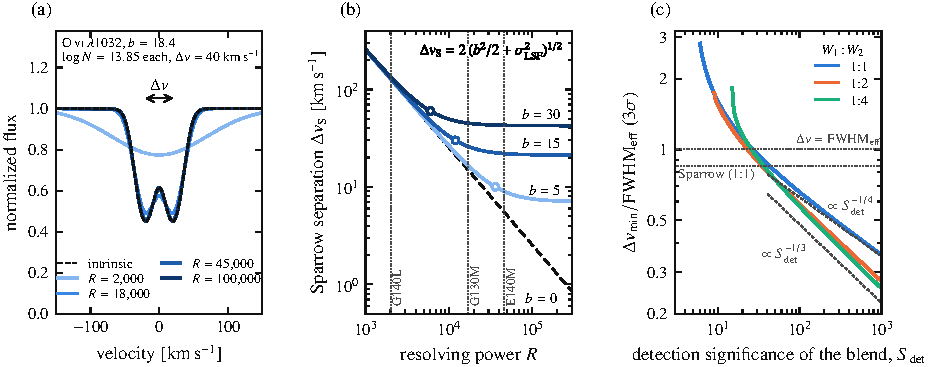
\includegraphics[width=\textwidth]{lsf_resolution.pdf}
\caption{How the LSF limits component separation. (a) Two \OVI{} components before and after convolution. (b) Sparrow separation versus $R$; circles mark $R_k$. (c) Universal 3$\sigma$ resolution limit for optically thin pairs with equivalent-width ratios 1:1, 1:2 and 1:4.}\label{fig:lsf}\end{figure*}
\begin{figure*}[p]\centering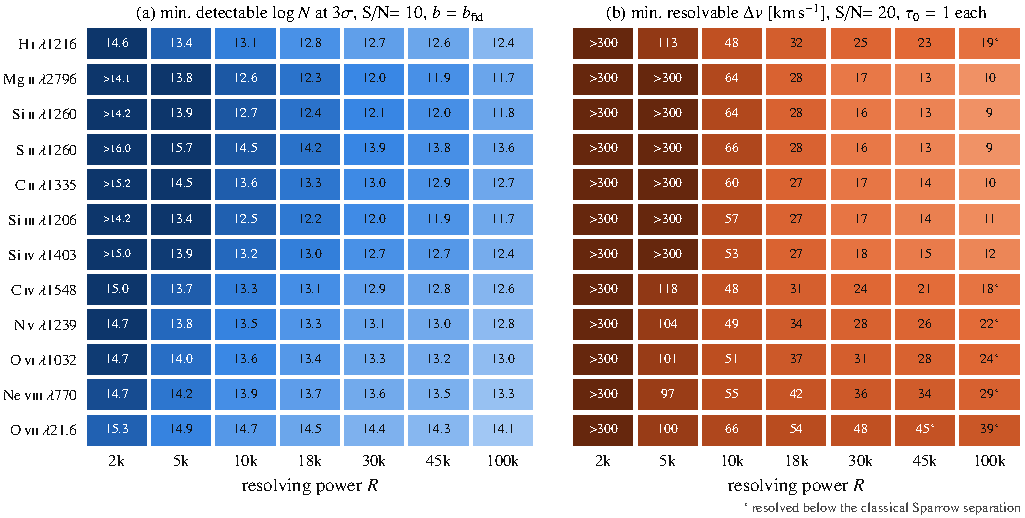
\includegraphics[width=\textwidth]{requirements_matrix.pdf}
\caption{Requirement matrix for twelve transitions. (a) Minimum detectable $\log N$ at S/N\,=\,10 and $b=b_{\rm fid}$. (b) Smallest resolvable separation for two equal $\tau_0=1$ components at S/N\,=\,20.}\label{fig:matrix}\end{figure*}
\begin{figure*}[p]\centering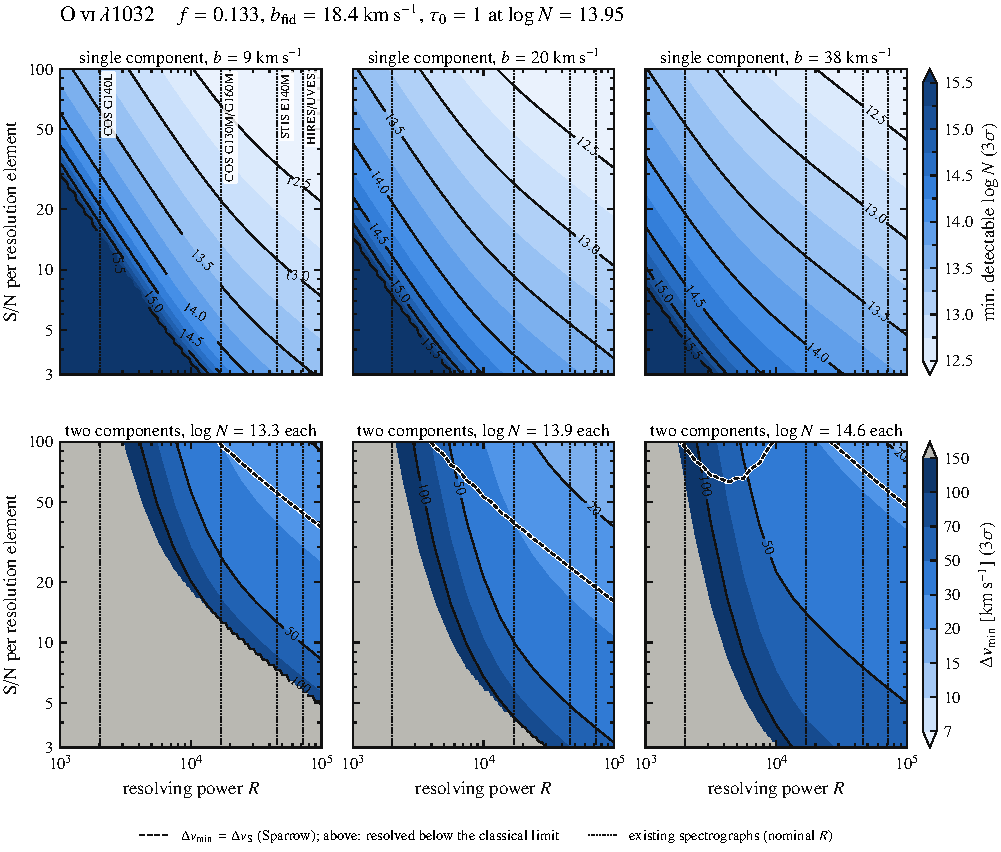
\includegraphics[width=\textwidth]{OVI1032_instrument_plane.pdf}
\caption{\OVI\,$\lambda1032$ in the instrument plane. Top: minimum detectable $\log N$ for three $b$. Bottom: smallest resolvable separation for two equal components at three column densities. Inside the dashed contour, pairs are resolved below the Sparrow separation.}\label{fig:ovi}\end{figure*}
\begin{figure*}[p]\centering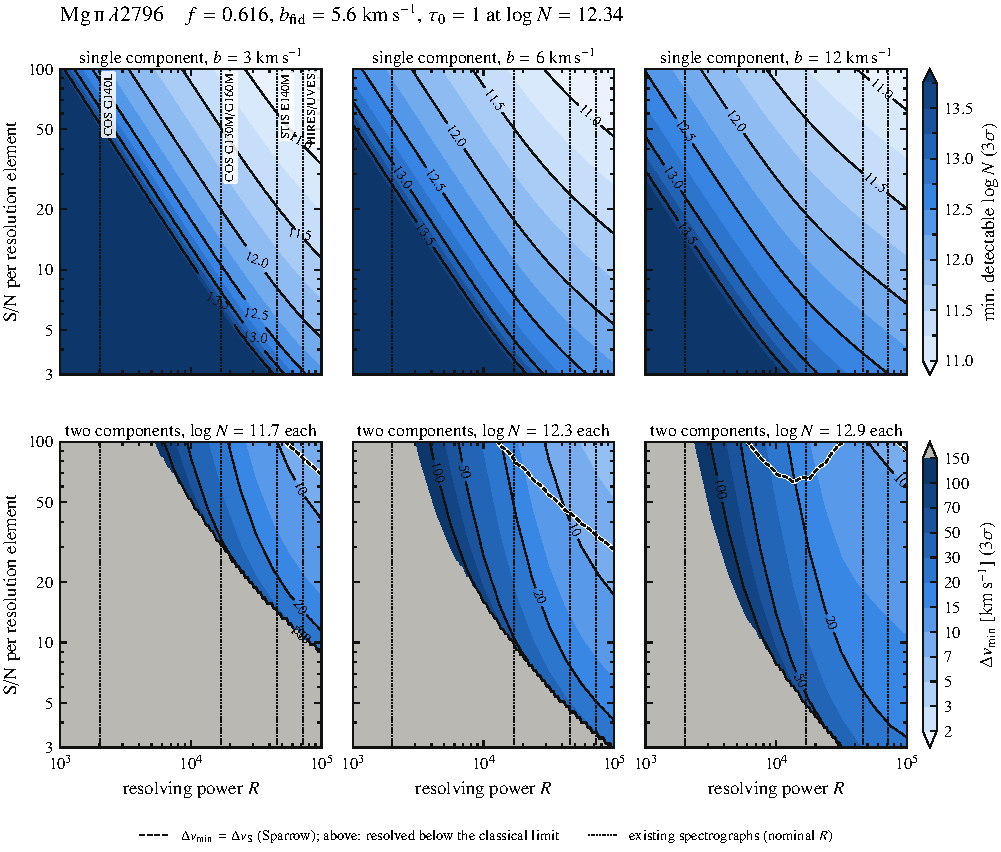
\includegraphics[width=\textwidth]{MgII2796_instrument_plane.pdf}
\caption{As Fig.~\ref{fig:ovi} for \MgII\,$\lambda2796$.}\label{fig:mgii}\end{figure*}
\end{document}
